%% Bemærk:
%%          Programmeringssprog skrives med stort begyndelsesbogstav (første gang fed, (hvis gennemgående))
%%          Pakker skrives med kursiv (\emph{})
{
{\sffamily Dette kapitel har til formål at gennemgå, hvordan
principperne fra kapitel \ref{chap_indledning} og metoderne fra kapitel
\ref{chap_detektion} er blevet implementeret, samt hvilke problemer, der
kan opstå i denne forbindelse. Vi vil også komme ind på, hvordan
resultater --- som dem vist i kapitel \ref{chap_afproevning} ---
repræsenteres og gemmes, samt på hvordan vi kører analysen på malerierne
i vores database.  Vi forklarer programmet, og metoderne deri, ``fra
bunden og op'', dvs. at vi bevæger os fra lille kompleksitet, hvor der
lægges ud med de helt grundlæggende strukturer og principper, til stor
kompleksitet, når de enkelte dele sættes sammen.  I bilag
\ref{appendix_struktur} er vedlagt en oversigt over programmets opdeling.
Indledningsvis kigger vi på, hvilke programmeringssprog og biblioteker
vi benytter os af.
}

\section{Programmeringssprog og biblioteker\label{section_programmeringssprog}}
{
{\sffamily Ved valg af programmeringssprog har vi først og fremmest lagt
vægt på at kunne udarbejde en prototype hurtigt og bruge et sprog, som
er let at gå til. Det valgte sprog skal også gøre det nemt at udvide den
endelige implementation. Vi har også gerne villet undgå at skulle
konstruere komplicerede datastrukturer for relativt simple metoder, både
af hensyn til tidspresset og til implementationens kompleksitet. Af
ovenstående grunde har vi besluttet at udarbejde vores løsning i
programmeringssproget \textbf{Python}\cite{PythonLanguage}. Vores
erfaring er, at dette sprog er yderst velegnet at skrive forholdsvis
avancerede prototyper i.
}

\subsection{OpenCV}
Til udførelse af billedmanipulationer benytter vi os af et bibliotek
skrevet i C og C++, der hedder \emph{OpenCV}\cite{OpenCV}. Biblioteket
er udviklet af Intel og tilbyder, udover et solidt udvalg af algoritmer,
bindinger til Python\cite{OpenCVPython}. Endelig er det meget
veldokumenteret og giver referencer til publikationer om bibliotekets
algoritmer. Biblioteket er udviklet med specielt henblik på real-tids
behandling af billeder, f.eks. med et videokamera som kilde, men det
egner sig også til brug på enkelte billeder.  \emph{OpenCV} tilbyder
mange brugbare datastrukturer med hensyn til arbejdet med billeder i
Python.

Der er også andre biblioteker til billedbehandling i Python. Her kan
nævnes \emph{PIL} (Python Imaging Library)\cite{PIL} og
\emph{PythonMagick} (ImageMagick bindings)\cite{PMck}, men de er ikke
nær så grundige som \emph{OpenCV}.

\subsubsection{Andre muligheder}
Der er to helt oplagte muligheder, med hensyn til programmeringssprog,
når man taler om billedbehandling, nemlig Matlab\cite{MatlabLang} og
dets Open Source-alternativ Octave\cite{Octave}. Disse sprog blev dog
valgt fra, da vores samlede erfaring med udvikling i disse sprog ikke
var stor nok.  Endvidere finder vi, at disse sprog, på trods af, at de
især egner sig til den type beregninger, vi skal lave, er besværlige at
lave større programmer med. Matlab og Octave er dog blevet brugt til at
sammenligne resultater og teste alternative metoder med.

Da \emph{OpenCV} er skrevet i C/C++, ville det også være oplagt at bruge
et af disse sprog. Vores erfaring er dog, at man let kommer til at bruge
mere tid på at konstruere de fornødne datastrukturer og hjælpemetoder,
end på at fokusere på opgavens kerne. En senere implementation, med
fokus på køretid, kunne med fordel implementeres i C/C++, da man så
ville have fuld kontrol over, hvilke strukturer der bliver brugt i
programmet.

\subsection{Værktøjer til databasen}
Vi bruger \textbf{SQLite}\cite{Sqlite} til selve databasen, hovedsagelig
fordi der ikke kræves nogen videre konfiguration af en sådan database.
Den underliggende database er dog underordnet, da vi bruger
Python-pakken \emph{SQLObject}\cite{Sqlobject}, som giver et
abstraktionslag til en bred vifte af databaser. Vi opretter blot de
tabeller, vi ønsker at have i databasen, som klasser i Python og får
ligeledes en sådan klasse tilbage, når der laves forespørgsler til
databasen. Da \emph{SQLObject} klarer al kommunikation med databasen, er
det derfor muligt at skifte den underliggende database ud, hvis man
ønsker det. SQLite har endvidere den umiddelbare fordel, at selve
databasen eksisterer som en fil i filsystemet.  Det er derfor en let sag
at tage sikkerhedskopier af databasen uden alt for meget besvær.

\subsection{Andre værktøjer}
Vi har gjort brug af statistikprogrammet \textbf{R}\cite{Rlang} til at
behandle og præsentere vores resultater i kapitel \ref{chap_resultater}.
Da programmet primært er blevet brugt som hjælpeværktøj, til at
producere grafer, vil vi ikke komme nærmere ind på, hvordan disse
hjælpeprogrammer er blevet udviklet.

}

% vim: set tw=72 spell spelllang=da:


\section{Billedbehandling med OpenCV\label{section_impBilledbehandling}}
{
{\sffamily I det følgende, kaster vi et detaljeret blik på
billedbehandlingsmetoderne i programmet. Efter en teknisk
introduktion til digitale billeder, vises hvilke datastrukturer og
metoder \emph{OpenCV} stiller til rådighed, og hvordan disse bruges, til
at udtrække regioner i digitale billeder. Endeligt vil vi undersøge,
hvilke svagheder vores implementation, til udtrækning af regioner, har.
}

\subsection{Digitale billeder}
I afsnit \ref{section_kort_intro} blev der givet en kort introduktion
til den digitale repræsentation af billeder. Vi antog, at en pixel kunne
antage værdier i mængden $\{0, 1\}$. I praksis, kan pixels godt tage
andre værdier. Vi arbejder med billeder, hvor værdien for hver pixel, er
repræsenteret ved tre 8 bit størrelser --- hver især med værdier i
mængden $\{0, 1, 2, \cdots, 254, 255\}$. Sammensætningen af de tre
værdier, som beskrives som kanaler eller farvebånd, kaldes for en
RGB-farve, hvor tallene repræsenteret ved $(R,G,B)$ angiver mængden af
hhv. rød, grøn og blå farve i en pixel. Et sådant billede, kaldes for et
RGB-billede. Vores korpus består af sådanne RGB-billeder med 8 bits, og
vi benytter derfor også denne repræsentation internt. Der er enkelte
undtagelser, hvor der kun bruges én kanal, således at vi arbejder med
gråtonebilleder. For en uddybende forklaring om billeders
repræsentation, refereres igen til \cite{SIOlsen}.

\marker{Hvordan repræsenteres billeder i \emph{OpenCV}? Skriv det
her.}{Husk det!}
Noget med matricer og arrays og Python og \emph{OpenCV}.

\subsection{Resultaters struktur\label{resultat_struktur}}
Indledningsvist vil vi introducere nogle vigtige datastrukturer, som vi
bruger fra \emph{OpenCV}. Alle datastrukturer og metoder fra
\emph{OpenCV}, er prefikset med ``cv'', hvilket gør det let, at skelne
vores egne metoder fra dem der er givet i \emph{OpenCV}.  Der
præsenteres i det følgende en notation for datastrukturer.  Notationen
er underlagt strukturen vist i \eqref{types_class}.
\begin{multline}
    \textbf{class~} [\textit{name}] = \{ \\
    \shoveleft{\qquad[\textit{type}] : [\textit{varName}]} \\
    \shoveleft{\}}\shoveright{}
    \label{types_class}
\end{multline}
I \eqref{example_class} ses et eksempel på en struktur kaldet
\textbf{ExampleClass}.
\begin{multline}
    \textbf{class~} \textrm{ExampleClass} = \{ \\
    \shoveleft{\qquad\textbf{int} : \textit{intValue}} \\
    \shoveleft{\qquad\textbf{string} : \textit{stringValue}} \\
    \shoveleft{\qquad\textbf{int[2]} : \textit{arrayValues}} \\
    \shoveleft{\}}\shoveright{}
    \label{example_class}
\end{multline}
Når en type har et suffiks på formen $\textit{type}[i]$, hvor $i$ er et
heltal, betyder det, at dette er en liste af længde $i$ af typen
\textit{type}.  Bemærk, at en strukturs navn bliver skrevet med fed
skrift i brødteksten, når der refereres til en sådan. Ligeledes vil en
strukturs navn blive skrevet med fed i pseudokoden, hvis der refereres
til den. Vi kan definere en ny struktur \textbf{NewClass}, som viser
dette, i \eqref{new_class} herunder.
\begin{multline}
    \textbf{class~} \textrm{NewClass} = \{ \\
    \shoveleft{\qquad\textbf{ExampleClass} : \textit{exampleInstance}} \\
    \shoveleft{\qquad\textbf{string} : \textit{stringValue}} \\
    \shoveleft{\}}\shoveright{}
    \label{new_class}
\end{multline}
Vi vil nu beskrive de vigtigste datastrukturer, som vi bruger, med
ovenstående notation.

\subsubsection{cvScalar}
Strukturen \textbf{cvScalar} fungerer egentlig blot som en almindelig
liste med værdier. En instans af \textbf{cvScalar} kan dog kun indeholde
1, 2, 3 eller 4 værdier. Strukturen vist i \eqref{cvScalar_class} har fire
værdier.
\begin{multline}
    \textbf{class~} \textrm{cvScalar} = \{ \\
    \shoveleft{\qquad\textbf{double[4]} : \textit{value}} \\
    \shoveleft{\}}\shoveright{}
    \label{cvScalar_class}
\end{multline}
I \emph{OpenCV}, og vores implementation i øvrigt, bruges strukturen
blandt andet til RGB-farver og tærskelværdier. Til RGB-værdier bruger
\emph{OpenCV} også strukturen \textbf{CV\_RGB}, men dette er reelt blot
en instans af \textbf{cvScalar}.

\subsubsection{cvPoint}
Strukturen \textbf{cvPoint} har til formål at beskrive punkter i det
to-dimensionelle plan. Den er givet i \eqref{cvPoint_class}.
\begin{multline}
    \textbf{class~} \textrm{cvPoint} = \{ \\
    \shoveleft{\qquad\textbf{int} : \textit{x}} \\
    \shoveleft{\qquad\textbf{int} : \textit{y}} \\
    \shoveleft{\}}\shoveright{}
    \label{cvPoint_class}
\end{multline}
Strukturen er simpel, men er en meget central del af implementationen.
Den bruges blandt andet til at angive snit i billedet samt fortælle
floodfill hvor vi skal male og skifte farve.

\subsubsection{cvRect}
Denne struktur beskriver et rektangel, ved at angive dets øverste venstre
hjørne og dimensioner. Strukturen vises i \eqref{cvRect_class}.
\begin{multline}
    \textbf{class~} \textrm{cvRect} = \{ \\
    \shoveleft{\qquad\textbf{int} : \textit{x}} \\
    \shoveleft{\qquad\textbf{int} : \textit{y}} \\
    \shoveleft{\qquad\textbf{int} : \textit{height}} \\
    \shoveleft{\qquad\textbf{int} : \textit{width}} \\
    \shoveleft{\}}\shoveright{}
    \label{cvRect_class}
\end{multline}
I vores implementation af den naive fremgangsmåde, som nævnt i afsnit
\ref{section_naiv}, er det denne struktur, som angiver en regions
begrænsende rektangel. Vi vil i afsnit \ref{section_vurdering_regioner},
se hvordan strukturen \textbf{cvRect} bruges, til at vurdere, om regioner
ligger i det gyldne snit.

\subsubsection{cvConnectedComp}
\emph{OpenCV} har en implementation af den floodfill-metode beskrevet i
afsnit \ref{subsec_floodfill}. Vi vil komme nærmere ind på denne senere,
men den nævnes nu, da den gør brug af en datastruktur kaldet
\textbf{cvConnectedComp}. Denne struktur bruges, til at beskrive den
region i billedet, som floodfill fylder ud.  Strukturen er vist i
\eqref{cvConnectedComp_class}.
\begin{multline}
    \textbf{class~} \textrm{cvConnectedComp} = \{ \\
    \shoveleft{\qquad\textbf{double} : \textit{area}} \\
    \shoveleft{\qquad\textbf{float} : \textit{value}} \\
    \shoveleft{\qquad\textbf{cvRect} : \textit{rect}} \\
    \shoveleft{\}}\shoveright{}
    \label{cvConnectedComp_class}
\end{multline}
Strukturen indeholder en regions begrænsende rektangel og regionens
areal.

\subsubsection{Resultater}
Vi vil nu introducere en ny struktur, som repræsenterer Pythons
\emph{dictionary}, forkortet \emph{dict}.  En \emph{dict} viser vi som i
\ref{def_dict}.
\begin{eqnarray}
    \langle[\textit{dictName}]\rangle = \{ [\textit{key}] : [\textit{data}] \}
    \label{def_dict}
\end{eqnarray}
Som et simpelt eksempel, kan vi konstruere en \emph{dict}
$\angles{LuckyNumbers}$, som indeholder personers lykketal:
% TeX-Gods, please forgive me :(
\begin{multline}
    \angles{LuckyNumbers} = \{ \qquad \textrm{Tom Cruise} : 4 , \\
    \textrm{Arthur Dent} : 42 \qquad\qquad\\
    \shoveleft{\}}\shoveright{}
    \label{lucky_dict}
\end{multline}
% In honor of the danish Tom Cruise
Data i en \emph{dict}, kan godt være af mere komplicerede typer, f.eks.
kan man have en anden \emph{dict}. Man kan således lave en hierakisk
struktur, som egner sig opbevaring af fundne regioner i et billede. Vi
ønsker at have hierakiet vist i figur \ref{resultat_hieraki}.

\begin{figure}[!h]
    \dirtree{%
    .1 $\textrm{ImageRegions}$ .
    .2 $\textrm{RatioRegions}$ .
    .3 $\textrm{CutRegions}$ .
    .4 $region0$ .
    .4 $region1$ .
    .4 $region2$ .
    .2 $\textrm{RatioRegions}$ .
    .3 $\textrm{CutRegions}$ .
    .2 $\textrm{RatioRegions}$ .
    .2 \dots .
    }
    \caption[]{Hierakisk struktur til resultater}
    \label{resultat_hieraki}
\end{figure}

Vi har, at et billede kan have et endeligt antal snitratioer, som man
ønsker at undersøge. Disse snitratioer, har enten to eller fire snit,
som nævnt i afsnit \ref{section_opdeling}. I disse snit er der et
endeligt antal fundne regioner. Vi repræsenterer hver node i figur
\ref{resultat_hieraki} med en \emph{dict}. På nederste niveau har vi
selve regionen, som floodfill-metoden har lagt i strukturen
\textbf{cvConnectedComp}. Vi ønsker dog også, at gemme hvilken farve,
regionen er blevet tildelt i det segmenterede billede. Vi gemmer derfor
parret $(color, region)$, som er instanser af henholdsvis
\textbf{CV\_RGB} og \textbf{cvConnectedComp}. Hver region bliver tildelt
et \emph{id}, som er en strengrepræsentation af regionens farve.  Hvis
det antages, at regionens farve er hvid, vil den have RGB-værdien $(255,
255, 255)$ og den får derfor tildelt $id = \textrm{'255255255'}$.
Regioners id er kun unikt for et givet snit. Vi konstruerer nu
$\angles{CutRegions}$, som indeholder de fundne regioner for et snit.
$\angles{CutRegions}$ er vist herunder i \eqref{CutRegions_dict}.
\begin{multline}
    \angles{CutRegions} = \{ \textit{~RegionId} : \\
    (\textbf{CV\_RGB~}\textit{color}, \textbf{cvConnectedComp~}\textit{region}) \}\quad
    \label{CutRegions_dict}
\end{multline}

\noindent I $\angles{CutRegions}$ bruges regionens id som nøgle. Vi kan nu
konstruere den \emph{dict} i niveauet over som vi betegner
$\angles{RatioRegions}$. Den ses i \eqref{RatioRegions_dict}.
\begin{eqnarray}
    \angles{RatioRegions} = \{ \textit{~CutNo} : \angles{CutRegions} \}
    \label{RatioRegions_dict}
\end{eqnarray}

\noindent $\angles{RatioRegions}$ holder alle regioner for en givet
snitratio.  Hvert snit, tilknyttet en snitratio, blev i afsnit
\ref{section_opdeling}, tildelt et id i mængden $\{0,1,2,3\}$. Vi bruger
snittets id som nøgle.  Data i $\angles{RatioRegions}$ er den instans af
$\angles{CutRegions}$ som tilhører snittet.

Det sidste niveau i hierakiet fra figur \ref{resultat_hieraki}, er endnu
en \emph{dict} givet ved $\angles{ImageRegions}$ vist i
\eqref{ImageRegions_dict}.
\begin{eqnarray}
    \angles{ImageRegions} = \{ \textit{~CutRatio} : \angles{RatioRegions} \}
    \label{ImageRegions_dict}
\end{eqnarray}

\noindent $\angles{ImageRegions}$ har nøglen $CutRatio$, som angiver en
snitratio til et billede. Hver snitratio har et antal snit, som endeligt
har et antal fundne regioner. Vi har således fået beskrevet den
struktur, som resultater bliver repræsenteret ved.

Resultatet fra en analyse på et billede, med snitratioerne $0.5$ og
$0.618$, ligner da det nedenstående:
%% !!! Bwadr-tex !!!
\begin{multline}
    \angles{ImageRegions} = \{ 0.5 : \{ 0 : \{ \textrm{'012345678'} : (color, region) \},\\
                                            \{ \textrm{'123456789'} : (color, region) \}
                                            \},\\
                                            \{ 1 : \{ \textrm{'012345678'} : ( \cdots ) \}, 
                                            \{ \cdots \} \}, \\
                              0.618 : \{ 0 : \{ \cdots \} \}, \{ 1 :
                              \cdots \}, \{ 2 : \cdots \}, \{ 3 : \cdots
                              \} \\
    \shoveleft{\}}\shoveright{}
    \label{CutRegions_dict}
\end{multline}

\subsection{Udtrækning af regioner}
I afsnit \ref{sammensaetning_af_metoder} er der givet en overordnet
fremgangsmåde, for at trække regioner ud af billedet, i forhold til et
givet snit. Resten af dette afsnit, vil omhandle den egentlige
implementation af denne fremgangmåde og problemerne tilknyttet.
Indledningsvist vises, hvordan snit i billedet repræsenteres.

\subsubsection{Repræsentation af snit i billedet}
Vi tidligere, i afsnit \ref{section_opdeling}, argumenteret for, hvordan
vi finder det gyldne snit i et billede. Det er nævnt, at man ikke
nødvendigvis behøver at betragte det gyldne snit, men vi kan arbejde med
helt arbitrære snit. Vi vil derfor blot referere til \emph{snit i
billedet}, da den enkelte snitratio er underordnet. Metoderne i dette
afsnit er ikke specifikke for snitratioen $\varPhi$, men kan overføres
til ethvert andet snit i billedet, med en arbitrær snitratio.

Snit i et billede bliver imidlertid --- meget intuitivt --- blot
repræsenteret ved et linjestykke. Vi præsenterer nu datastrukturen
\textbf{Line}, som består af et linjestykkes to endepunkter.
\begin{multline}
    \textbf{class~} \textrm{Line} = \{ \\
    \shoveleft{\qquad\textbf{cvPoint} : \textit{p1}} \\
    \shoveleft{\qquad\textbf{cvPoint} : \textit{p2}} \\
    \shoveleft{\}}\shoveright{}
    \label{Line_class}
\end{multline}
Strukturen er simpel, men fleksibel, og lader mulighederne stå åbne,
for, i en anden implementation, at betragte andet end blot vand- og
lodrette snit i billedet.

\subsubsection{Præparation af billedet}
Det første skridt i præparation af billedet, inden udtrækningen af
regioner, er at detektere kanterne på objekter i billedet.  Som nævnt i
afsnit \ref{udtraek_kanter}, bruger vi kantdetektionsmetoden Canny.
\emph{OpenCV} har implementeret denne metode som \texttt{cvCanny}.
Metoden skal køres på et sort/hvid-billede, så vi starter med at lave en
sort/hvid kopi af det originale billede. Vi skal også bruge et tomt
output-billede, hvori kanterne kan indtegnes. Dette skal ligeledes være
et sort/hvid-billede. Resultatet fra \texttt{cvCanny} er tidligere vist
i figurene \ref{canny_kanter} og \ref{sammen_kanter}.

I andet skridt af fremgangsmåden sløres billedet, så vi tillader
floodfill-metoden at dække et større areal. \emph{OpenCV} stiller
metoden \texttt{cvSmooth} til rådighed, for sløring af billeder.
\texttt{cvSmooth} tager følgende argumenter: det oprindelige billede, et
billede hvori resultatet vises, dimensionerne på foldningsmatricen der
skal bruges samt hvilken sløringsmetode der ønskes brugt. Metoderne vist
i afsnit \ref{udtraek_sloering} er til rådighed ved at bruge
konstanterne \texttt{CV\_BLUR}, \texttt{CV\_GAUSSIAN} og
\texttt{CV\_MEDIAN}. Inden vi detekterer kanter i et billede, bruger vi
simpel sløring, da vi på denne måde kun betragter kanter, som fremstår
tydeligt i billedet.  Simpel sløring er hurtigt og effektiv, og bliver
derfor også brugt på billedet inden vi bruger floodfill-metoden.

Sidste skridt, inden den egentlige segmentering og udtrækning af
regioner, er fremhævelse af de detekterede kanter. Kanterne skal
fremhæves, da den simple sløringsmetode kan have visket nogle de
originale kanter ud.  Vi ønsker stadig, at kunne begrænse
floodfill-metoden, så vi kan holde regioner i billedet adskilt. Kanterne
fremhæves ved at oprette et nyt billede, med samme størrelse som
originalbilledet. Alle pixels, i det nye billede, farves sort. Alle
pixels, fra det originale billede, kopieres over i det nye billede, med
undtagelse af pixels, hvorpå der er detekteret en kant. Derved bliver
pixels med en kant, ikke farvet, dvs.  de forbliver sorte. At lade
kanterne være sorte kan have nogle utilsigtede konsekvenser. Vi henviser
til afsnit \ref{subsec_svagheder} for en gennemgang af disse.

\subsubsection{Segmentering ved floodfill-metoden}
Vi beskriver nu metoden, til at trække regioner ud af et billede, der er
blevet præpareret som beskrevet ovenfor. Metoden bygger videre på
beskrivelsen givet i \ref{sammensaetning_af_metoder}, hvor
floodfill-metoden bruges på hver pixel langs et snit. I praksis er denne
fremgangsmåde meget langsom, især på store billeder. Vi vil derfor komme
frem til en metode, som kun bruger floodfill-metoden på de nødvendige
pixels.  Vi starter med, at forklare en meget naiv algoritme, som vi
løbende videreudvikler, for at komme frem til den endelige fremgangsmåde
for at trække regioner ud, af et præpareret billede. \emph{OpenCV} har
implementeret floodfill-metoden som \texttt{cvFloodFill} og det er denne
vi bruger, til at markere regioner i billedet.

Informationerne fra et kantdetekteret billede, kan hjælpe
\texttt{cvFloodFill} til at segmentere et billede, for endeligt at
trække regioner ud af dette. Hvis vi har et snit, repræsenteret ved en
instans af strukturen \textbf{Line}, kan vi gemme punkterne, hvor en
kant krydser snittet. Et eksempel, ses i figur
\ref{impUdtraek_kantpunkter}, hvor vi har et horisontalt snit,
repræsenteret ved linjestykket $AB$, og punkterne $e_1, \cdots, e_6$ er
der hvor en kant krydser. Vi antager i det følgende, at pixels, i
billedet vi undersøger, har RGB-værdier i mængden
$\{(0,0,0),(255,255,255)\}$, hvilket vil sige, at billedets pixels enten
er helt sorte eller helt hvide --- billedet vi undersøger er binært.

\begin{figure}[p]
    \centering
    \begin{picture}(240,30)
        \put(0, 10){$A$}
        \put(3, -5){\line(0, 1){10}}

        \put(82, 10){$e_1$}
        \put(85, 0){\circle*{3}}

        \put(102, 10){$e_2$}
        \put(105, 0){\circle*{3}}

        \put(134, 10){$e_3$}
        \put(137, 0){\circle*{3}}

        \put(158, 10){$e_4$}
        \put(161, 0){\circle*{3}}

        \put(200, 10){$e_5$}
        \put(203, 0){\circle*{3}}

        \put(221, 10){$e_6$}
        \put(224, 0){\circle*{3}}

        \put(233, 10){$B$}
        \put(236, -5){\line(0, 1){10}}

        \put(3, 0){\line(1, 0){233}}
    \end{picture}
    \caption[]{Punkter, hvor der er en kant der krydser snittet.}
    \label{impUdtraek_kantpunkter}
\end{figure}

\begin{figure}[p]
    \centering
    \begin{picture}(240,30)
        \color{red}
        \put(3, 0){\line(1, 0){81}}

        \color{green}
        \put(85, 0){\line(1, 0){20}}

        \color{blue}
        \put(105, 0){\line(1, 0){32}}

        \color{cyan}
        \put(137, 0){\line(1, 0){24}}

        \color{purple}
        \put(161, 0){\line(1, 0){42}}

        \color{orange}
        \put(203, 0){\line(1, 0){21}}

        \color{violet}
        \put(224, 0){\line(1, 0){12}}

        \color{black}

        \put(0, 10){$A$}
        \put(3, -5){\line(0, 1){10}}

        \put(82, 10){$e_1$}
        \put(85, 0){\circle*{3}}

        \put(102, 10){$e_2$}
        \put(105, 0){\circle*{3}}

        \put(134, 10){$e_3$}
        \put(137, 0){\circle*{3}}

        \put(158, 10){$e_4$}
        \put(161, 0){\circle*{3}}

        \put(200, 10){$e_5$}
        \put(203, 0){\circle*{3}}

        \put(221, 10){$e_6$}
        \put(224, 0){\circle*{3}}

        \put(233, 10){$B$}
        \put(236, -5){\line(0, 1){10}}

    \end{picture}
    \caption[]{Farvede linjestykker. \colbox{red}{$Ae_1$},
    \colbox{green}{$e_1e_2$}, \colbox{blue}{$e_2e_3$},
    \colbox{cyan}{$e_3e_4$}, \colbox{purple}{$e_4e_5$},
    \colbox{orange}{$e_5e_6$}, \colbox{violet}{$e_6B$}.
    }
    \label{impUdtraek_naiv_res}
\end{figure}

\begin{lstlisting}[caption={Naiv pseudokode til segmentering af binære
    billeder.},captionpos=b,label={naiv_segmentering},numbers=left,
    frame=single, breaklines=false, float=p]
for lineSegment in Cut:
    # Get a new color that is not in the component dictionary
    color = getRandomColor()
    region = cvConnectedComp()

    center = getCenter(lineSegment)

    cv.cvFloodFill(img, center, color, lowerThres, upperThres, region)

\end{lstlisting}

\begin{lstlisting}[caption={Original pseudokode til udtrækning af
    regioner. Denne kan returnere den samme region flere
    gange.},captionpos=b,label={pseudo_udtraek_org},numbers=left,
    frame=single, breaklines=false, float=h]
for lineSegment in Cut:
    # Get a new color that is not in the component dictionary
    color = getRandomColor()
    region = cvConnectedComp()

    for pixel in lineSegment:

        # Check if the color of the pixel equals current color
        if not (color(pixel) ==  color):

            # Check if the color of the pixel are in the saved regions
            if not (color(pixel) in CutRegions):
                cv.cvFloodFill(img, pixel, color, lowerThres, upperThres, region)

    # Color the last pixel again to make sure that
    # the returned component is the entire region
    cv.cvFloodFill(img, pixel, color, lowerThres, upperThres, region)

    # Put the results in the CutRegions-dictionary
    CutRegions[color.toString()] = (color, region)
\end{lstlisting}

\suppressfloats
\clearpage

Som vist i figur \ref{impUdtraek_kantpunkter}, kan snittet opdeles i
mindre linjestykker. Nu antager vi meget naivt, at punkterne på
linjestykket $Ae_1$ tilhører én region, mens punkterne på $e_1e_2$
tilhører en anden region, og så fremdeles. Med denne antagelse, samt
antagelsen om at billedet er binært, kan vi, for hvert linjestykke
mellem kanter, bruge \texttt{cvFloodFill} en enkelt gang. Hver gang vi
passerer en kant, maler \texttt{cvFloodFill} med en ny tilfældig farve.
Således skelnes regioner fra hinanden. \texttt{cvFloodFill} kaldes,
bland andet, med en en instans af \textbf{cvConnectedComp}, hvori den
netop farvede region lægges. Vi bruger \texttt{cvFloodFill} på midten af
hvert linjestykke og tildeler linjestykkerne tilfældige farver, som vist
i figur \ref{impUdtraek_naiv_res}. Pseudokode for fremgangsmåden vises i
kodeboks \ref{naiv_segmentering}.

Denne fremgangsmåde virker fint i det et-dimensionelle plan på binære
billeder, som i figur \ref{impUdtraek_naiv_res}, men i to dimensioner,
opstår der problemer med antagelsen om, at hvert linjestykke tilhører
sin egen region. Vi betragter nu figur \ref{region_extract}, hvor
\ref{region_init} er det oprindelige billede.  Snittet i figur
\ref{impUdtraek_kantpunkter} rammer altså de tre sorte kasser i figur
\ref{region_init}. Vi gennemgår nu iterationerne i fremgangsmåden fra
kodeboks \ref{naiv_segmentering}, på billedet i \ref{region_init}.
Disse er vist i figurene \ref{region1} til \ref{region7}.

\begin{enumerate}
    \item Linjestykket $Ae_1$ bliver malet rødt. Hele den hvide baggrund
        males rød og denne region returneres.
    \item Linjestykket $e_1e_2$ males. Den første kasse fra venstre
        bliver malet grøn. Denne region returneres.
    \item Linjestykket $e_2e_3$ males blåt, men dette er den samme region som
        fundet i første iteration. Der returneres alligevel en ny
        region.
    \item Linjestykket $e_3e_4$ males lyseblåt og udgøres af den
        midterste kasse, der returneres som en ny region.
    \item Linjestykket $e_4e_5$ bliver malet og endnu engang findes en
        region som vi allerede har fundet.
    \item Linjestykket $e_5e_6$ males orange og vi finder den sidste
        kasse.
    \item Linjestykket $e_6B$ males lilla og vi returnerer igen en
        allerede fundet region.
\end{enumerate}
Vi ender altså med at have returneret syv regioner, ligesom antallet af
linjestykker, men når vi kigger på resultatet, i figur \ref{region7}, er
der kun fire forskellige farver. Vi returnerer den samme region, den som
i originalen var hvid, i alt fire gange. Vi vil gerne undgå denne
opførsel, og gemmer derfor de fundne regioner, sammen med den farve
regionen er blevet tildelt. Således kan vi kontrollere farven på den
pixel vi står til at male, inden vi bruger \texttt{cvFloodFill}. Hvis
denne pixel har en farve lig en allerede returneret region, undlader vi
at male denne, da vi antager, at denne pixel er del af en allerede
returneret region.

\begin{figure}[!p]
    \setlength\fboxsep{0pt}
    \setlength\fboxrule{0.5pt}
    \centering
    \subfloat[Original]{
        \label{region_init}
        \fbox{
\includegraphics[width=0.4\textwidth]{afsnit/implementation/billeder/billedbehandling/binary_init}}}\hspace{1em}
    \subfloat[1. iteration]{
        \label{region1}
        \fbox{
\includegraphics[width=0.4\textwidth]{afsnit/implementation/billeder/billedbehandling/binary_s1}}}\\
    \subfloat[2. iteration]{
        \label{region2}
        \fbox{
\includegraphics[width=0.4\textwidth]{afsnit/implementation/billeder/billedbehandling/binary_s2}}}\hspace{1em}
    \subfloat[3. iteration]{
        \label{region3}
        \fbox{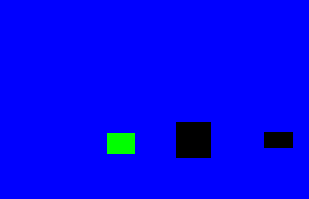
\includegraphics[width=0.4\textwidth]{afsnit/implementation/billeder/billedbehandling/binary_s3}}}\\
    \subfloat[4. iteration]{
        \label{region4}
        \fbox{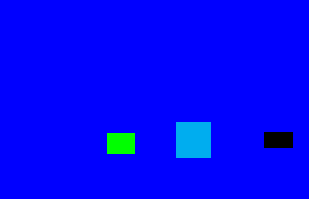
\includegraphics[width=0.4\textwidth]{afsnit/implementation/billeder/billedbehandling/binary_s4}}}\hspace{1em}
    \subfloat[5. iteration]{
        \label{region5}
        \fbox{
\includegraphics[width=0.4\textwidth]{afsnit/implementation/billeder/billedbehandling/binary_s5}}}\\
    \subfloat[6. iteration]{
        \label{region6}
        \fbox{
\includegraphics[width=0.4\textwidth]{afsnit/implementation/billeder/billedbehandling/binary_s6}}}\hspace{1em}
    \subfloat[7. iteration]{
        \label{region7}
        \fbox{
\includegraphics[width=0.4\textwidth]{afsnit/implementation/billeder/billedbehandling/binary_s7}}}
        \caption[]{Iterationerne for kodeboks \ref{naiv_segmentering}}
    \label{region_extract}
\end{figure}

Kompleksiteten stiger, når vi ikke har med binære billeder at gøre. Som
vist i kapitel \ref{chap_afproevning}, så vil vi, på grund af
tærskelværdierne til \texttt{cvFloodFill} og \texttt{cvCanny}, ikke
nødvendigvis finde de samme regioner med de to metoder. Vi ønsker at
bruge kanterne, til at indikere en ny region, så det er ikke nok, at bruge
\texttt{cvFloodFill} på midten af et linjestykke mellem kanter. I figur
\ref{floodfill_taerskel_problem} er problemet illustreret, hvor sorte
streger er detekterede kanter og lyseblå indikerer den region vi har
fundet. Hvid farve er pixels, som endnu ikke er blevet farvet af
\texttt{cvFloodFill}.  Bemærk, at linjestykket, fra kanten af billedet
til den næste detekterede kant, som krydser snittet, \emph{ikke} er
blevet farvet helt lyseblå. Dette viser, at det ikke er ligemeget på
hvilken pixel vi bruger \texttt{cvFloodFill} på linjestykker mellem
kanter. Vi ønsker derfor, at male enhver pixel, på et givet linjestykke,
som \emph{endnu ikke er blevet farvet af \texttt{cvFloodFill}}.

\begin{figure}[p]
    \setlength\fboxsep{0pt}
    \setlength\fboxrule{0.5pt}
    \centering
    \fbox{
\includegraphics[width=0.8\textwidth]{afsnit/implementation/billeder/billedbehandling/floodfill_color.png}}
    \caption[]{Problemet med floodfill-metoden i billeder med flere
    farver. Hvid farve er ikke blevet malet af floodfill-metoden endnu.
    Den lyseblå region dækker ikke hele linjestykket.}
    \label{floodfill_taerskel_problem}
\end{figure}

Fremgangsmåden, for at udtrække regioner ved et snit i et arbitrært
billede, er vist i kodeboks \ref{pseudo_udtraek_org}. Metoden tager
højde for den tidligere gjorte observation, hvor en allerede fundet
region bliver overskrevet. Regioner gemmes i $\angles{CutRegions}$ på
linje 20, som opretter en ny indgang med regionens id som nøgle.
Regionens id fåes ved kaldet \texttt{color.toString()}. Ved
inspektion ses det dog, at denne fremgangsmåde lider under nøjagtig
samme svaghed som fremgangsmåden brugt i figur \ref{region_extract}.

Under udviklingen af metoden i kodeboks \ref{pseudo_udtraek_org},
opdagede vi, at det ikke altid var hele regionen der blev returneret fra
\texttt{cvFloodFill}. Vi betragter nu figur \ref{new_reg_small_box},
hvor vi har udvidet den lyseblå region fra figur
\ref{floodfill_taerskel_problem}. Regionen som bliver lagt i instansen
af \textbf{cvConnectedComp}, er den \emph{senest udfyldte}. Derfor får vi
faktisk kun returneret et undersæt, af de pixels, som udgør den lyseblå
region.

\begin{figure}[p]
    \setlength\fboxsep{0pt}
    \setlength\fboxrule{0.5pt}
    \centering
    \subfloat[En tilføjelse til den lyseblå region. Det begrænsende
    rektangel svarer kun til udvidelsen.]{
        \label{new_reg_small_box}
        \fbox{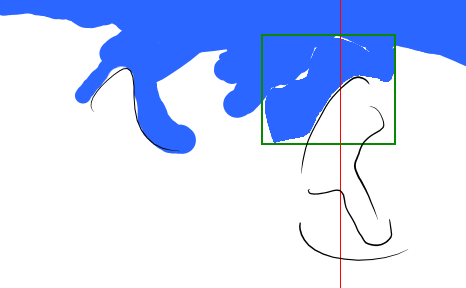
\includegraphics[angle=0,width=0.8\textwidth]{afsnit/implementation/billeder/billedbehandling/floodfill_color_new_reg_small_box}}
        }\\
    \subfloat[Ved at bruge floodfill på regionen igen, markeres hele den
    lyseblå region, som vi ønsker.]{
        \label{new_reg_big_box}
        \fbox{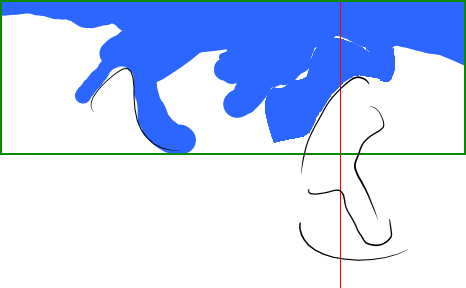
\includegraphics[angle=0,width=0.8\textwidth]{afsnit/implementation/billeder/billedbehandling/floodfill_color_new_reg_big_box}}
        }
    \caption[]{
    Floodfills opførsel ved udvidelse af regioner.
    }
    \label{floodfill_return_entire_region}
\end{figure}

Problemet i \ref{new_reg_small_box} løses ved at bruge
\texttt{cvFloodFill} en ekstra gang. Derfor blev kaldet til
\texttt{cvFloodFill} i linje 17 tilføjet. Man bruger derfor
\texttt{cvFloodFill} igen på den sidste pixel af linjestykket, da dette
vil returnere hele regionen, som vist i
figur \ref{new_reg_big_box}. Kaldet gør dog også, at der \emph{altid}
bliver returneret en region for hvert segment. Dette er ikke
ønskværdigt, specielt ikke hvis vi er sprunget over alle pixels på et
linjestykke. Dette sker, netop når hele regionen allerede er blevet fyldt
ud. Fejlen i linje 17 har eksisteret selv under vores kørte eksperiment
i \marker{ref}{Husk husk husk}.
Vi har fjernet duplikaterne på databaseniveau, men metoden er senere
blevet rettet til at have den korrekte opførsel. Den reviderede metode
er vist i kodeboks \ref{pseudo_udtraek_rev}.

\begin{lstlisting}[caption={Revideret pseudokode til udtrækning af
    regioner. Returnerer ingen
    duplikater.},captionpos=b,label={pseudo_udtraek_rev},numbers=left,
    frame=single, breaklines=false, float=p]
for lineSegment in Cut:
    # Get a new color that is not in the component dictionary
    color = getRandomColor()

    # Set region to None, as we have not yet found any
    region = None

    for pixel in lineSegment:

        # Check if the color of the pixel equals current color
        if not (color(pixel) ==  color):

            # Check if the color of the pixel are in the saved regions
            if not (color(pixel) in CutRegions):
                # Now we've got a new region
                region = cvConnectedComp()
                cv.cvFloodFill(img, pixel, color, lowerThres, upperThres, region)

                # Color the pixel again to make sure that
                # the returned component is the entire region
                cv.cvFloodFill(img, pixel, color, lowerThres, upperThres, region)

    # If we have found a region, then put the result in the CutRegions-dictionary
    if not (region is None):
        CutRegions[color.toString()] = (color, region)
\end{lstlisting}

Metoden i kodeboks \ref{pseudo_udtraek_rev} bruger \texttt{cvFloodFill}
to gange, hver gang man møder en ikke-farvet pixel. Dette koster lidt
køretid, men sikrer, at man altid får hele regionen returneret i
\textbf{cvConnectedComp}. Man kan fristes til at flytte kaldet i linje
21 ind i \texttt{if}-sætningen i linje 24, men dette åbner op for
svagheden igen, da vi ikke ved, om den sidste pixel tilhører den
aktuelle region. Derfor er vi nødt til at ofre lidt køretid, for at
være sikre på resultatet. Metoden benytter et ``først til
mølle''-princip, hvor en pixel, når den først et blevet tilknyttet en
region, altid vil tilhøre denne.

Pseudokoden i kodeboks \ref{pseudo_udtraek_rev} trækker dog kun de
regioner ud som rører snittet. I kapitel \ref{chap_detektion} indførtes
et margin, således at også regioner, som ligger tæt på snittet, kan
trækkes ud. Vi vil nu udvide pseudokoden i kodeboks
\ref{pseudo_udtraek_rev} til også at trække regioner ud, som krydser
margin. Vi navngiver metoden \texttt{ExtractRegions}, og den tager et
snit som argument. Metoden ses i kodeboks
\ref{pseudo_udtraek_margin}. Metoden trækker først regioner ud med
hensyn til det nedre margin, så med hensyn til det øvre margin og til
sidst med hensyn til selve snittet. Alle regioner gemmes i den samme
instans af $\angles{CutRatios}$. For selve udregningen af margin,
henvises til afsnit \ref{subsec_margin_udregning}.

\begin{lstlisting}[caption={Pseudokode til udtrækning af regioner med
    margin.},captionpos=b,label={pseudo_udtraek_margin},numbers=left,
    frame=single, breaklines=false, float=h]
def ExtractRegions(cut):
    # Calculate lowerMargin and upperMargin
    (lowerMargin, upperMargin) = calculateMargins(cut)
    Cuts = [lowerMargin, upperMargin, cut]

    # Initialize an empty CutRegions-dict
    CutRegions = {}

    for Cut in Cuts:
        for lineSegment in Cut:
            # Get a new color that is not in the component dictionary
            color = getRandomColor()

            # Set region to None, as we have not yet found any
            region = None

            for pixel in lineSegment:

                # Check if the color of the pixel equals current color
                if not (color(pixel) ==  color):

                    # Check if the color of the pixel are in the saved regions
                    if not (color(pixel) in CutRegions):
                        # Now we've got a new region
                        region = cvConnectedComp()
                        cv.cvFloodFill(img, pixel, color,
                                    lowerThres, upperThres, region)

                        # Color the pixel again to make sure that
                        # the returned component is the entire region
                        cv.cvFloodFill(img, pixel, color,
                                    lowerThres, upperThres, region)

            # If we have found a region,
            # then put the result in the CutRegions-dictionary
            if not (region is None):
                CutRegions[color.toString()] = (color, region)

    return CutRegions
\end{lstlisting}

\subsection{Svagheder\label{subsec_svagheder}}
Den endelige metode, for udtrækning af regioner, med hensyn til et givet
snit i billedet, har nogle svagheder, som bør nævnes. Den første er
allerede nævnt i den foregående sætning: Metoden trækker kun regioner ud
\emph{med hensyn} til et snit. Dette betyder, at kun regioner, som rører
margin eller selve snittet, bliver trukket ud. Foregående skal tages
helt bogstaveligt, i den forstand, at vi \emph{skal} have, at en region
har en pixel enten på det nedre margin, det øvre margin eller på selve
snittet, for at blive trukket ud. Vi kan altså godt have interessante
regioner, som faktisk har mindst én kant af sit begrænsende rektangel
inden for margin, som ikke bliver trukket ud.  Dette er tilfældet, hvis
\emph{to kanter} af det begrænsende ligger indenfor snittet, og
regionens form og størrelse i øvrigt opfylder kravene for en interessant
region. Et eksempel er vist i figur \ref{respect_to_cut}, hvor den sorte
region ikke vil blive trukket ud, selvom den har to kanter inden for
margin. Denne opførsel er beklagelig, men kan faktisk løses trivielt.
\note{Dette er måske ikke skide-smart at skrive,
men det er et vagt forsøg på at dække over egen inkompetence. Skal vi
rette koden igen?}
Det overlades som opgave til læseren, at modificere pseudokoden i
kodeboks \ref{pseudo_udtraek_margin}, så den kan udtrække regioner med
begge kanter inden for margin.
Når regioner kun trækkes ud, med hensyn til et snit, kan vi ved denne
metode heller ikke garantere en fuld segmentering af billedet.

\begin{figure}[p]
    \setlength\fboxsep{0pt}
    \setlength\fboxrule{0.5pt}
    \centering
    \fbox{
\includegraphics[width=0.8\textwidth]{afsnit/implementation/billeder/billedbehandling/respect_to_cut.png}}
    \caption[]{Sort region, som ikke bliver trukket ud af billedet.
    Selvom regionens begrænsende rektangel ligger inden for margin, så
    krydser regionen hverken nedre margin, øvre margin eller selve
    snittet. Derfor opdages regionen ikke.}
    \label{respect_to_cut}
\end{figure}

\subsubsection{Valg af tilfældige RGB-værdier}
Man skal endvidere være opmærksom på, at hver gang vi markerer en ny
region, vælges en tilfældig farve til denne.  Vi kan, i vores valg af
farve, være uheldig og vælge en, som bliver brugt i det originale
billede. Når vi kalder \texttt{cvFloodFill} igen, for at være sikre, at
hele regionen bliver returneret, kan vi smelte to regioner sammen, som
egentlig ikke burde hænge sammen. I figur \ref{floodfill_colors} er
denne situation vist på det prærarerede billede fra figur \ref{bathers}.
I samme forbindelse skal vi være opmærksomme på, at vi ligeledes kan
være uheldige, at støde på en pixel, som har en farve lig med en
allerede farvet region. I dette tilfælde, vil denne pixel blive anset
som værende del af en eksisterende region, hvilket resulterer i at vi
ikke bruger \texttt{cvFloodFill} på denne. Vi kan dog håbe, at denne
pixel bliver inkluderet i den efterfølgende iteration --- hvis den næste
pixels farve, da ikke er lig en allerede udvalgt regions, og denne
ligger inden for den tilladte afvigelse, for \texttt{cvFloodFill}.  Vi
vælger aldrig, at farve en region med en farve som allerede er brugt til
en region, men vi kan også her være uheldige og vælge en farve, som
ligger inden for floodfill-metodens tilladte afvigelse.

\begin{figure}[p]
    \setlength\fboxsep{0pt}
    \setlength\fboxrule{0.5pt}
    \centering
    \subfloat[Originalt præpareret billede inden vi vælger en tilfældig
    farve til floodfill.]{
        \label{colors_1}
        \fbox{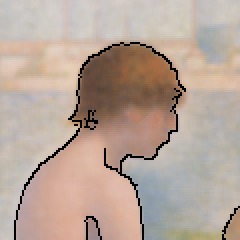
\includegraphics[width=0.3\textwidth]{afsnit/implementation/billeder/billedbehandling/pre_floodfill_1}}}\hspace{1em}
    \subfloat[Region fyldes med farve lig eksisterende pixels i
    billedet. Pixels i drengens hår har nu samme farve som kroppen.]{
        \label{colors_2}
        \fbox{
\includegraphics[width=0.3\textwidth]{afsnit/implementation/billeder/billedbehandling/pre_floodfill_2}}}\\
    \subfloat[Når floodfill bruges en ekstra gang, for at være sikker på
    at hele regionen returneres, smeltes drengens krop og hår sammen.]{
        \label{colors_3}
        \fbox{
\includegraphics[width=0.3\textwidth]{afsnit/implementation/billeder/billedbehandling/pre_floodfill_3}}}\hspace{1em}
    \subfloat[Hvis den første region havde fået en anden farve, ville vi
    ikke have smeltet to regioner sammen.]{
        \label{colors_4}
        \fbox{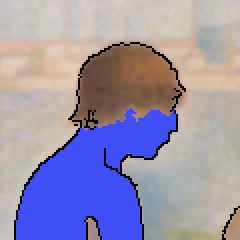
\includegraphics[width=0.3\textwidth]{afsnit/implementation/billeder/billedbehandling/pre_floodfill_4}}}\\
    \label{floodfill_colors}
    \caption[]{Uheldige valg af tilfældig farve til regioner.}
\end{figure}

\subsubsection{Ikke-sammenhængende regioner}
Metoden i kodeboks \ref{pseudo_udtraek_margin}, trækker højest én region
ud per segment. Dette giver mening, set i lyset af hvad
udtrækningsmetoden er blevet udviklet til, nemlig udtrækning af
\emph{sammenhængende regioner} afgrænset ved kantdetektion. I afsnit
\ref{section_computer_betragter} antog vi, at interessante regioner i et
billede, er tydeligt afgrænset. En region er ikke tydeligt afgrænset,
hvis vi faktisk \emph{har} flere regioner indenfor et segment. I figur
\ref{usammenhaengende_region} betragter vi en hypotetisk situation, hvor
en region ikke har været tydeligt afgrænset. Billedet i figur
\ref{usammenhaengende_region}, illustrerer et billede, som allerede er
blevet segmenteret ved metoden i kodeboks \ref{pseudo_udtraek_margin}.
De sorte cirkler markerer dér, hvor vi har fundet kanter, som krydser
snittet. Vi har altså fem segmenter på snittet. På det længste segment,
ser vi, at den mørkeblå region er blevet afbrudt af en tidligere fundet
region. Den mørkeblå region er således ikke sammenhængende. Metoden
returnerer kun den nederste mørkeblå region, da vi ikke kan få forbundet
de to mørkeblå regioner. Vi mister derfor informationen om at der
faktisk befinder sig en region i midten af billedet.

Denne opførsel, er en konsekvens af vores antagelse, om at interessante
regioner er tydeligt afgrænset. Vi accepterer derfor, at situationen i
figur \ref{usammenhaengende_region} kan forekomme, og at vi derfor kan
undlade at trække enkelte regioner ud.

\begin{figure}[t]
    \setlength\fboxsep{0pt}
    \setlength\fboxrule{0.5pt}
    \centering
    \fbox{
\includegraphics[width=0.8\textwidth]{afsnit/implementation/billeder/billedbehandling/usammenhaengende_region.png}}
    \caption[]{Et segmenteret billede. Sorte cirkler angiver steder,
    hvor vi har detekteret en kant, der krydser snittet. Den mørkeblå
    region er usammenhængende over snittet, da den afbrydes af den røde
    region. Kun den nederste mørkeblå region er blevet returneret.}
    \label{usammenhaengende_region}
\end{figure}

\subsubsection{Usikkerhed ved fremhævelse af kanter}
Endeligt skal vi nævne problemerne tilknyttet måden, vi fremhæver kanter
i et billede på. Som tidligere nævnt, så fremhæves kanterne, fordi vi
har sløret billedet med en metode, som kan udviske kanterne. De
fremhævede kanter tegnes i det slørede billede med sort farve.  Sort
farve vælges, uanset hvilke farver der er brugt i maleriet. Vi kan
derfor støde på problemer med mørke malerier eller lokalt i mørke
områder af et billede. Vi kan også være uheldige, at komme til at
forbinde to regioner, ved at markere kanterne med sort.

Vi valgte, at bruge sorte kanter, da dette var den hurtigste løsning på
daværende tidspunkt. Metoden \texttt{cvFloodFill} gør det faktisk
muligt, at bruge en maske, som, i mangel af et passende dansk ord, kan
bekrives som digital malertape. Man kan kalde \texttt{cvFloodFill} med
et kantdetekteret billede, således at man ikke maler over de steder i
billedet, hvor der er detekteret en kant. \emph{OpenCV} gør det dog
yderst besværligt, at bruge denne funktion, da det kantdetekterede
billede skal være to pixel større, i hver dimension --- det
kantdetekterede billede skal have en ramme på én pixel. At indsætte en
ramme burde være trivielt, men viste sig i praksis at være meget
besværligt. En meget naiv løsning, hvor pixels kopieres én ad gangen,
var tidskrævende på store billeder og vi beholdt derfor de sorte kanter.
Alternativt kunne man beskære det originale billede, men vi besluttede
at vi ikke ville manipulere med dimensionerne på vores inddata og bevare
det originale billede.

\subsection{Andre tilgange}
Dette afsnit vil kort nævne andre fremgangsmåder, vi har prøvet, for at
trække regioner ud af et billede. Vi har tidligt i udviklingen af
programmet, eksperimenteret både med Octave og Matlab. Til at starte
med, har vi brug disse sprog til at komme problemstillingen nærmere,
og udvikle naive implementationer af enkelte algoritmer.

I præparationen af billedet, inden udtrækning af regioner, vil vi gerne
have, at farverne i billedet bliver ensartede, men vi ønsker også at
bibeholde kanterne. Vi forsøgte at bruge en metode i \emph{OpenCV} der
hedder \texttt{cvPyrMeanShiftFiltering}, som netop segmenterer billedet
efter hvilke farver der ligner hinanden, men en fejl i biblioteket
forsagede altid en segmenteringsfejl i det underliggende C-program. Vi
blev siden gjort opmærksom på en sløringsmetode af Perona og
Malik\cite{perona1990scale}, hvor det grafiske resultat tilnærmer sig
det ønskede. Kun i Octaves \emph{Image}-pakke er denne implementeret. Vi
lavede en hurtig afprøvning, hvor resultatet fra denne metode blev
analyseret, men på basis at det endelige resultat, vurderede vi, at vi
godt kunne nøjes med at fremhæve kanterne i billedet efter en simpel
sløring.

Vi har også eksperimenteret med, først at skallere billedet ned, inden
man trak regioner ud. Dette gør nemlig, at kanterne forbliver intakte,
mens farverne, til en vis grad, bliver mere ensartede. Vi stødte dog på
problemer når billedet skulle skalleres op igen, eller rettere, få
resultaterne skalleret op, så de passede til originalbilledet. Vi mister
også meget præcision, når vi bruger et nedskalleret billede til at finde
regioner i.

}

%\begin{figure}[!h]
%    \centering
%    \begin{picture}(240,30)
%        \color{black}
%        \put(0, 10){$A$}
%        \put(233, 10){$B$}
%
%        \linethickness{5mm}
%        \put(85, 0){\line(1, 0){20}}
%
%        \linethickness{9mm}
%        \put(137, 3){\line(1, 0){24}}
%
%        \linethickness{3mm}
%        \put(203, 3){\line(1, 0){21}}
%
%        \linethickness{0.2mm}
%        \put(3, -5){\line(0, 1){10}}
%
%        \put(236, -5){\line(0, 1){10}}
%
%        \put(3, 0){\line(1, 0){233}}
%    \end{picture}
%    \caption[]{Eksempel på regioner der krydser snittet.}
%    \label{impUdtraek_regioner_snit}
%\end{figure}

% vim: set tw=72 spell spelllang=da:


\section{Vurdering af regioner\label{section_vurdering_regioner}}
{
{\sffamily Vi vender nu opmærksomheden mod selve implementationen af de
metoder, som afgør, hvorvidt en udtrukket regionen er interessant, samt
hvordan vi har implementeret den naive fremgangsmåde, som bedømmer, om
en region ligger i det gyldne snit. Alle metoder vedrørende vurdering af
regioner er implementeret i filen \texttt{regionSelector.py} i mappen
\texttt{lib/}.  Vi har igen, at metoderne ikke er specifikke for det
gyldne snit, men kan anvendes på ethvert snit i billedet. Sidst i
afsnittet viser vi, hvordan vi har implementeret den udvidede vurdering.
Vi starter med at se på en fælles datastruktur, som bruges, når regioner
bliver vurderet.
}

\subsection{Datastruktur til betingelser}
Når vi skal afgøre, hvorvidt et antal udtrukne regioner er interessante
og ligger i snittet, er der en række betingelser, der skal være opfyldt.
Til disse, er der forbundet nogle udregninger, som vil være de samme for
hver region. Vi bruger derfor en struktur, som indeholder resultaterne
fra disse udregninger, således at de ikke skal udføres for hver eneste
region vi kontrollerer. Datastrukturen kaldes \textbf{Constraints} og
ses herunder i \eqref{Constraints_class}.
\begin{multline}
    \textbf{class~} \textrm{Constraints} = \{ \\
    \shoveleft{\qquad\textbf{int} : \textit{coordinate}} \\
    \shoveleft{\qquad\textbf{double} : \textit{minSize}} \\
    \shoveleft{\qquad\textbf{double} : \textit{minMass}} \\
    \shoveleft{\qquad\textbf{int[}2\delta + 1\textbf{]} : \textit{acceptRange}} \\
    \shoveleft{\}}\shoveright{}
    \label{Constraints_class}
\end{multline}
Variablene \texttt{minSize} og \texttt{minMass} relaterer sig kun til
klassificering af \emph{interessante regioner}, mens \texttt{coordinate}
og \texttt{acceptRange} hører til klassificering af regioner,
\emph{liggende i snittet}. De enkelte variable vil, i det følgende,
blive forklaret nærmere, når det er relevant.

\subsection{Interessante regioner}
Til at afgøre om udtrukket region er interessant, bruges definition
\ref{def_interessant}. Bemærk, at vurderingen af interessante regioner,
ikke har noget at gøre med hverken snitratio eller margin. Vi undersøger
udelukkende de udtrukne regioners areal og masse. Regioner bliver
vurderet, umiddelbart efter de er blevet trukket ud, så vi har
regionerne til rådighed, som en instans af $\angles{CutRegions}$. Vi
definerer nu to metoder; én til at kontrollere en regions størrelse og
én til at kontrollere dens masse. Vi kalder disse \texttt{checkSize} og
\texttt{checkMass}. De kan ses i kodeboks \ref{pseudo_size_mass}.

\begin{lstlisting}[caption={Metoder til at konstollere en regions
    størrelse og masse.},captionpos=b,label={pseudo_size_mass},
    frame=tb, breaklines=false, float]
def checkSize(component, constraints):
    "Test if the component have size greater than the minumum size
    defined by the constraints."
    return component.area >= constraints.minSize

def checkMass(component, constraints):
    "Check if the component have mass greater than the minimum mass
    defined by the contraints."
    rect = component.rect
    mass = component.area/(rect.width * rect.height)
    return mass >= constraints.minMass
\end{lstlisting}

Metoderne i kodeboks \ref{pseudo_size_mass}, returnerer begge en
sandhedsværdi, for hvorvidt en region lever op til betingelserne, for en
interessant region. Vi vil imidlertid gerne kontrollere hver enkelt
region, så vi konstruerer en ny metode, som returnerer en \emph{dict}
kun med de interessante regioner.  Metoden, kaldet
\texttt{GetInterestingRegions}, ses i kodeboks
\ref{pseudo_GetInterestingRegions}. Den tager, som argument, den instans
af $\angles{CutRegions}$, som returneres fra \texttt{ExtractRegions}, se
kodeboks \ref{pseudo_udtraek_margin}.

\begin{lstlisting}[caption={Metode som returnerer kun de insteressante
    regioner, givet en instans af $\angles{CutRegions}$}, captionpos=b,
    label={pseudo_GetInterestingRegions}, frame=tb, breaklines=false,
    float]
def GetInterestingRegions(CutRegions, constraints):
    interestingRegions = {}
    for id in CutRegions:
        component = CutRegions[id][1]
        passSizeCheck = checkSize(component, constraints)
        passMassCheck = checkMass(component, constraints)
        if (passSizeCheck and passMassCheck):
            interestingRegions[id] = CutRegions[id]
    return interestingRegions
\end{lstlisting}

I kodeboks \ref{pseudo_GetInterestingRegions} bruger vi en instans af
\textbf{Constraints} som argument til metoderne, som kontrollerer
regionens størrelse og masse. Vi skal derfor, inden metoden
\texttt{GetInterestingRegions} kaldes, have initialiseret vores
betingelser, så de passer til billedet. I kapitel
\ref{chap_afproevning}, blev fastsat en procentsats for en regions
minimumareal i forhold til billedets størrelse, og denne
minimumstørrelse findes ved udregningen i \eqref{region_min_size}
herunder.
\begin{equation}
    \mathtt{minSize} =
    \lfloor
    \mathrm{minSizePercentage}\cdot\mathrm{height}\cdot\mathrm{width}
    \rfloor
    \label{region_min_size}
\end{equation}
Ligeledes, har vi fastsat en procentsats for en regions minimummasse, men denne
skal vi ikke regne videre på, da metoden \texttt{checkMass} også regner
en procentsats ud for den givne region. Vi gemmer den fastsatte
procentsats, for regioners minimummasse direkte i vores instans af
\textbf{Constraints}. I \texttt{checkMass} sammenlignes minimummassen
med regionen masse direkte.

\clearpage
\subsection{Naiv vurdering af regioner}
Vi vil nu se på, hvordan den naive fremgangsmåde vurderer hvorvidt en
region, ligger i det gyldne snit. Definition \ref{def_naiv} siger, at en
region mindst skal have én kant inden for margin, så vi vil først give
en forklaring på, hvordan dette margin bliver repræsenteret.

\subsubsection{Udregning af margin\label{subsec_margin_udregning}}
Størrelsen på margin er givet ved en procentsats $\Delta$.  Hvis vi kun
undersøger ét snit, bliver $\Delta$ sat til $2.4\%$ af billedets højde
eller bredde, alt efter hvilken orientering det aktuelle snit har.  Vi
har implementeret fastsættelsen af $\Delta$ således, at \emph{hvis} man
ønsker at sammenligne to snit, som ligger tættere på hinanden, end det
gyldne snit og to tredjedele, så findes den værdi af $\Delta$, der gør,
at disse snits margin ikke overlapper. I praksis gives en liste med
snitratioer, der ønskes undersøgt, og fra denne liste, findes den
mindste differens mellem ratioerne. Den mindste differens mellem
snitratioer, bruges da, som $\Delta$ for alle snit i analysen. Hvis den
mindste differens, mellem snitrationerne, er større end $2.4\%$, sættes
$\Delta$ til $2.4\%$.

Når vi skal vurdere regioner med hensyn til vores margin, får vi brug
for den eksakte pixelstørrelse på margin. I filen
\texttt{marginCalculator.py} i mappen \texttt{lib/} er der implementeret
metoder til dette. Her bruges metoden \texttt{getPixels}, som, givet et
billede, et snit og $\Delta$, returnerer afstanden fra
snittet til margin i pixels, som vi også skriver som $\delta$. I
\texttt{marginCalculator.py} finder vi også den mindste differens mellem
snitratioer, ved metoden \texttt{getPercentage}.

\begin{figure}[t]
    \centering
    \begin{picture}(122,55)
        \put(61, 50){$x$}
        \put(-10, 22){$y$}
        \put(0, 45){\circle*{3}}
        \put(-1, 45){\vector(1, 0){120}}
        \put(0, 45){\vector(0, -1){48}}

        \color{red}
        \put(88, 50){\line(0, -1){55}}

        \color{blue}
        \put(84, 50){\line(0, -1){55}}
        \put(92, 50){\line(0, -1){55}}

        \color{black}

        \put(66, 30){$-^{x}$}
        \put(78, 30){\vector(1, 0){20}}

        \put(100, 30){$+^{x} $}
        \put(98, 30){\vector(-1, 0){20}}


    \end{picture}
    \caption[]{Koordinatsystem med indtegnet snit og margin. Bemærk, at
    ved det vertikale snit, skal vi kun betragte regioners $x$-værdi,
    når vi skal bedømme om de ligger inden for margin. Således kan
    margin repræsenteres kun ved de tilladte $x$-værdier.}
    \label{margin_koordinatsystem}
\end{figure}
Vi udnytter, at vi enten betragter et vertikalt eller horisontalt snit.
Når vi har et vertikalt snit, behøver vi kun at betragte $x$-værdier, da
$y$-værdien ikke influerer på det vertikale snit. Omvendt med
horisontale snit, behøver vi kun at betragte $y$-værdier, da
$x$-værdierne, i denne situation, ikke har betydning for snittet.
Tilfældet, for det vertikale snit, er vist i figur
\ref{margin_koordinatsystem}.

Ovenstående gør, at vi nu kan oprette et sæt, bestående af de
koordinater, som ligger inden for margin. Hvis vi betragter et vertikalt
snit, kan vi i Python oprette sættet af accepterende $x$-værdier, ved at
bruge \texttt{range}. Vores implementation bruger endvidere variablen
\texttt{coordinate} i \textbf{Constraints}, som, lidt misvisende,
indikerer om snittet vi undersøger, er vertikalt eller horisontalt. Er
snittet vertikalt, sættes \texttt{coordinate} til \texttt{0}, og
\texttt{1} for et horisontalt snit. For ethvert snit, kan vi da finde de
accepterende $x$-værdier, som vist i kodeboks \ref{pseudo_acceptRange}.
Variablen \texttt{margin}, der tages som argument, er den
pixelstørrelse, der er returnet fra metoden \texttt{getPixels} fra
\texttt{marginCalculator.py}.

\begin{lstlisting}[caption={Metode som genererer sættet af accepterende
    koordinater.},captionpos=b,label={pseudo_acceptRange},
    frame=tb, breaklines=false, float]
GetAcceptRange(cut, margin, coordinate):
    if coordinate:
        # Horizontal cut
        lower_bound = cut.p1.y - margin
        upper_bound = cut.p1.y + margin
        acceptRange = range(lower_bound, upper_bound)
    else:
        # Vertical cut
        lower_bound = cut.p1.x - margin
        upper_bound = cut.p1.x + margin
        acceptRange = range(lower_bound, upper_bound)

    return acceptRange
\end{lstlisting}

\subsubsection{Kontrol på en regions begrænsende rektangel}
\begin{lstlisting}[caption={Metode, som kontrollerer, hvorvidt en region
    har en kant af det begrænsende rektangel inden for margin.},
    captionpos=b, label={pseudo_position}, frame=tb, breaklines=false,
    float]
def checkPosition(component, constraints):
    "Test if the component have a bounding box inside the accepting
    rectangle defined in the constraints."
    d = component.rect.width
    p = component.rect.x
    if constraints.coordinate:
        d = component.rect.height
        p = component.rect.y

    lowerInRange = p in constraints.acceptRange
    upperInRange = (p + d) in constraints.acceptRange

    return lowerInRange or upperInRange
\end{lstlisting}
Når vi har fastsat \texttt{coordinate} og fundet værdierne i
\texttt{acceptRange} kan vi kan afgøre, om en interessant region, ligger
placeret i snittet. Vi har allerede udnyttet, at vi kun behøver at
betragte én koordinat, og det er derfor ligetil, at kontrollere, om en
regions begrænsende rektangel, har en kant inden for margin. Regionen er
repræsenteret som en instans af \textbf{cvConnectedComp}, hvori der er
en instans af \textbf{cvRect}. Vi har en metode, kaldet
\texttt{checkPosition}, som, alt efter om vi har et vertikalt eller et
horisontalt snit, returnerer en sandhedsværdi for, om den relevante
koordinat findes i de accepterende koordinater. Metoden ses i kodeboks
\ref{pseudo_position}.

Vi kan nu sammensætte en metode, som returnerer alle interessante
regioner, med en kant inden for margin. Metoden tager en instans af
$\angles{CutRegions}$ og en instans af \textbf{Constraints} som
argumenter. Vi genererer altså vores betingelser inden vi begynder at
frasortere regioner, således at alle informationer om snittet og krav
for regioner ligger i instansen af \textbf{Constraints}. Den endelige
metode, for vurdering efter den naive fremgangsmåde, kaldes
\texttt{GetInterestingRegionsInCut} og er vist i kodeboks
\ref{pseudo_GetInterestingRegionsInCut}.

\begin{lstlisting}[caption={Pseudokode, som returnerer alle interessante
    regioner, der har en kant, af deres begrænsende rektangel, inden for
    margin.},
    captionpos=b, label={pseudo_GetInterestingRegionsInCut}, frame=tb, breaklines=false,
    float]
def GetInterestingRegionsInCut(CutRegions, constraints):

    # First remove uninteresting regions
    interestingRegions = GetInterestingRegions(CutRegions, constraints)

    # Initialize an empty dict
    interestingRegionsInCut = {}

    # Check every interesting region if it's bounding box
    # has an edge inside the margin
    for id in interestingRegions:
        component = interestingRegions[id][1]
        if checkPosition(component, constraints):
            interestingRegionsInCut[id] = interestingRegions[id]

    # The resulting dict contains only interesting regions
    # with an edge inside the margin
    return interestingRegionsInCut
\end{lstlisting}

\subsection{Udvidet vurdering af regioner}
Vi har også implementeret en udvidet vurdering af interessante
regioner. Grundprincipperne bag denne er gennemgået i afsnit
\ref{subsec_udvidet_massemidtpunkt}. Da vi ikke længere betragter en
regions begrænsende rektangel, men i stedet regionens form og
udstrækning, har brug vi for en anden måde, at repræsentere regionen på.
Vi tager derfor billedet, som \texttt{cvFloodFill} har arbejdet på, og
bruger dette til at approksimere regionens form.

\subsubsection{Approksimation af regioners form og udstrækning}
Fremgangsmåden for at approksimere en regions form og udstrækning er
simpel. Givet et segmenteret billede, fra \texttt{cvFloodFill}, og den
resulterende $\angles{CutRegions}$, fra \texttt{ExtractRegions}, kan vi,
for hver pixel i det begrænsende rektangel, kontrollere om denne har
samme farve, som regionen er blevet tildelt i segmentering af billedet.
Hvis farverne er ens, så gemmes dette punkt i en liste. Hvis regionen er
stor, kan dette godt være en tidskrævende procedure, så i praksis ønsker
vi ikke at kontrollere hver eneste pixel i det begrænsende rektangel. Vi
springer derfor et antal pixels over, for hver gang vi har kontrolleret
en pixel.  På denne måde får vi lavet et gitter, som vist i figur
\ref{grid}.  Pseudokode, for at approksimere en regions form og
udstrækning, er vist i kodeboks \ref{pseudo_GetRegionGrid}, som
definerer metoden \texttt{GetRegionGrid}, der returnerer en liste med
punkter for en region.

\begin{lstlisting}[caption={Metode til at approksimere en regions
    form. Bemærk linje 19, hvor der ses et eksempel på det omvendte
    koordinatsystem i \emph{OpenCV}.}, captionpos=b,
    label={pseudo_GetRegionGrid}, frame=tb,
    breaklines=false, float, numbers=left]
def GetRegionGrid(image, color, component, step):
    rect = component.rect

    # Initialize the area we want to traverse
    lower_x = rect.x
    lower_y = rect.y
    upper_x = lower_x + rect.width
    upper_y = lower_y + rect.height

    # Initialize an empty array
    coordinates = []

    # Traverse the bounding box with the defined step size
    for x in range(lower_x, upper_x, step):
        for y in range(lower_y, upper_y, step):

            # If we find a color in the image that equals the region
            # color, then we save that point
            if isSameColor(color, image[y][x]):
                coordinates.append(cvPoint(x, y))

    # Finally, return the resulting set of points
    return coordinates
\end{lstlisting}
% Sorry, I'm really sorry :(
Til senere brug, vil vi definere en metode, som finder en approksimation
til alle regioner i en instans af $\angles{CutRegions}$. Denne metode
returnerer en modificeret instans af $\angles{CutRegions}$, som vi
kalder for $\angles{CutGridRegions}$, således at den også indeholder
approksimationen til regionen. Strukturen er vist i
\eqref{CutGridRegions_dict}.
\begin{multline}
    \angles{CutRegions} = \{ \textit{~RegionId} : \\
    (\textbf{CV\_RGB~}\textit{color}, \textbf{cvConnectedComp~}\textit{region}, \textbf{cvPoint[]~}\textit{grid}) \}\quad
    \label{CutGridRegions_dict}
\end{multline}
Metoden \texttt{GridIt}, er vist i kodeboks \ref{pseudo_GridIt}, og går
alle regionerne igennem, mens den bygger den nye \emph{dict} op.

\begin{lstlisting}[caption={Metode, som finder approksimationen til alle
    regioner i en instans af $\angles{CutRegions}$.}, captionpos=b,
    label={pseudo_GridIt}, frame=tb,
    breaklines=false, float]
def GridIt(image, CutRegions, step):
    # Initialize an empty dict
    CutGridRegions = {}

    for id in CutRegions:
        # Get the color and component
        color = CutRegions[id][0]
        component = CutRegions[id][1]

        # Get the grid for the region
        grid = GetRegionGrid(image, color, component, step)

        # Save the findings
        CutGridRegions[id] = (color, component, grid)

    # Well, return
    return CutGridRegions
\end{lstlisting}

\subsubsection{Vurdering ved massemidtpunkt og udstrækning}
Definition \ref{def_expanded} fortæller os, at hvis en region har et
massemidtpunkt inden for margin og dens masse i øvrigt er jævnt fordelt
over snittet, så ligger denne i snittet.  En regions fordeling af masse
er givet i definition \ref{def_fordeling_ligning} og en regions
massemidtpunkt er givet i definition \ref{def_massemidtpunkt}. Vi skal
bruge approkimationen af regionens form og udstrækning til at afgøre om
regionen ligger i snittet.

Vi starter med at kigge på fordelingen af en regions masse, hvor vi skal
finde forholdet mellem punkter på højre og venstre side af snittet.
Metoden i kodeboks \ref{pseudo_distribution}, gør netop dette, og
returnerer en sandhedsværdi for, om regionens masse er jævnt fordelt
over snittet. Definition \ref{def_fordeling_procent} siger, at regionens
masse er jævnt fordelt over et snit, hvis forholdet mellem de to sider
er under $0.75$.  Metoden gør brug af snittets orientering, hentet i
$\textbf{Constraints}.\textit{coordinate}$, og det faktum, at vi kan
finde det midterste element i vores accepterende værdier, ved at tage
det $\left(\left\lfloor \frac{|\textit{acceptRange}|}{2}\right\rfloor +
1\right)$'te element i $\textbf{Constraints}.\textit{acceptRange}$.
Dette er selve snittet.

\begin{lstlisting}[caption={Metode som, på baggrund af regionens
    fordeling af masse, afgør, om denne region er jævnt fordelt},
    captionpos=b, label={pseudo_distribution}, frame=tb,
    breaklines=false, float]
def checkDistribution(grid, constraints):
    # If we've got no approximation, there's no distribution
    if len(grid) == 0:
        return False

    # Init variables for right/left-distribution as floats
    rDist = 0.0
    lDist = 0.0

    # Get the middle value of the accepting range, i.e. the cut
    middleIndex = floor(len(constraints.acceptRange)/2) + 1
    cutVal = constraints.acceptRange[middleIndex]

    # Check the position of every pixel in the grid
    for point in grid:
        if constraints.coordinate:
            # Horisontal
            if cutVal > point.y:
                left += 1
            elif cutVal < point.y:
                right += 1
        else:
            # Vertical
            if cutVal > point.x:
                left += 1
            elif cutVal < point.x:
                right += 1

    distribution = abs((lDist - rDist)/len(grid))
    return distribution < 0.75
\end{lstlisting}

Vi skal også bruge en metode, til at finde en regions massemidtpunkt.
Denne metode er vist i kodeboks \ref{pseudo_checkCenterOfMass} og
returnerer en sandhedsværdi for, hvorvidt en regions massemidtpunkt
befinder sig inden for margin.

\begin{lstlisting}[caption={Metode, som kontrollerer, om en regions
    massemidtpunkt er inden for margin.}, captionpos=b,
    label={pseudo_checkCenterOfMass}, frame=tb, breaklines=false,
    float]
def checkCenterOfMass(grid, constraints):
    if len(grid) == 0:
        return False

    sum = 0
    for point in grid:
        if constraints.coordinate:
            # Horisontal
            sum += point.y
        else:
            # Vertical
            sum += point.x

    centerOfMass = sum/len(grid)

    return centerOfMass in constraints.acceptRange
\end{lstlisting}

Endeligt samler vi alle metoderne, så vi kan sortere i alle resultaterne
returneret fra segmentering af billedet. Vi kalder denne metode for
\texttt{GetExpandedRegions} og viser denne i kodeboks
\ref{pseudo_GetExpandedRegions}.

\begin{lstlisting}[caption={Pseudokode, som returnerer alle interessante
    regioner, der er nævnt fordelt over snittet og har et massemidtpunkt
    inden for margin.},
    captionpos=b, label={pseudo_GetExpandedRegions}, frame=tb, breaklines=false,
    float]
def GetExpandedRegions(image, CutRegions, constraints):

    # First remove uninteresting regions
    interestingRegions = GetInterestingRegions(CutRegions, constraints)

    # Initialize the grid
    interestingRegions = GridIt(image, interestingRegions, constraints)

    # Initialize an empty dict
    interestingRegionsInCut = {}

    # Check every interesting region for center of mass
    # and distribution
    for id in interestingRegions:
        grid = interestingRegions[id][2]
        if checkDistribution(grid, constraints)
            and checkCenterOfMass(grid, constraints):
            interestingRegionsInCut[id] = interestingRegions[id]

    # The resulting dict contains only interesting regions
    # that qualify
    return interestingRegionsInCut
\end{lstlisting}

\clearpage

}

% vim: set tw=72 spell spelllang=da:


\section{Database\label{section_imp_database}}
{
Når vi har trukket regioner ud af billedet og vurderet dem efter
ovenstående simple algoritme kan vi stå tilbage med et egentligt
resultat. Vi ønsker at gemme dette resultat i en database så vi på et
senere tidspunkt kan bruge det i en samlet analyse af resultaterne.
Vi så i afsnit \ref{section_opbv_billeder} på et databaseskema til
opbevaring af maleriers metadata. Vi bygger nu videre på dette skema så
vi kan tilknytte resultater fra en analyse til de enkelte malerier. Det
fulde databaseskema ses nedenfor.

\begin{table}[!h]
    \centering
    \begin{tabular}{|l||c|c|c|c|c|c|}
        \hline
        \bf{artist} \hspace{0.5cm} & \underline{artistId} & name & born & died & school & timeline \\\hline
    \end{tabular}
    \caption{Databasetabel for kunstner}
    \label{artistTable}
\end{table}

\begin{table}[!h]
    \centering
    \begin{tabular}{|l||c|c|c|c|c|c}
        \hline
        \bf{painting} \hspace{0.5cm} & \underline{paintingId} & artistId & title & date & paint & $\cdots$ \\\hline
    \end{tabular}\\ \vspace{0.2cm}\hspace{1.2cm}
    \begin{tabular}{c|c|c|c|c|c|c}
        \hline
        $\cdots$ & material & location & url & form & type & $\cdots$ \\\hline
    \end{tabular}\\ \vspace{0.2cm}\hspace{1.4cm}
    \begin{tabular}{c|c|c|c|c|c|}
        \hline
        $\cdots$ & realHeight & realWidth & height & width & filepath \\\hline
    \end{tabular}
    \caption{Databasetabel for malerier}
    \label{paintingTable}
\end{table}

\begin{table}[!h]
    \centering
    \begin{tabular}{|l||c|c|c|c|c|c|c|}
        \hline
        \bf{run} \hspace{0.5cm} & \underline{runId} & trsh1 & trsh2 & lo & up & marginPercentage & method \\\hline
    \end{tabular}
    \caption{Databasetabel for en kørsel}
    \label{runTable}
\end{table}

\begin{table}[!h]
    \centering
    \begin{tabular}{|l||c|c|c|c|c|c|}
        \hline
        \bf{result} \hspace{0.5cm} & \underline{resultId} & runId & paintingId & cutRatio & cutNo & numberOfRegions \\\hline
    \end{tabular}
    \caption{Databasetabel for resultater}
    \label{resultTable}
\end{table}

\begin{table}[!h]
    \centering
    \begin{tabular}{|l||c|c|c|c|c|c|c|}
        \hline
        \bf{region} \hspace{0.5cm} & \underline{regionId} & resultId & x & y & height & width & area \\\hline
    \end{tabular}
    \caption{Databasetabel for regioner}
    \label{regionTable}
\end{table}

Tabellerne \ref{artistTable} og \ref{paintingTable} er de samme som vist
i afsnit \ref{section_opbv_billeder}, men er taget med her blot for at
vise databaseskemaet i sin helhed. Det øvrige databaseskema lægger vægt
på at minimere redundans og mulighed for at genskabe kørte analyser.
Sidstnævnte er vigtig osv\dots

}
% vim: set tw=72 spell spelllang=da:


\section{Kørsel\label{section_koersel}}
\textbf{Sæt sammen med database-afsnittet}\\
{
\subsection{Opbygning af en Kørsel}
Start.py er distributør af arbejde til de andre dele af programkoden.
Her følger en kort beskrivelse af hvad start.py gør og derefter kan ses
noget pseudokode for hvad gør.
Når en ny kørsel skal laves, skal der laves en ny python fil i
eksperiments mappen og denne skal importeres som environment.
Når alle indstillinger globale eller kørsels afhængige er blevet sat,
startes analysen på et enkelt billede. Dette gentages indtil at alle
billederne er blevet analyseret.

\begin{lstlisting}
cuts = environment.generateCuts()
environment.setSettings(settings)
environment.setGlobalSettings(globalSettings)
db = Database(globalSettings)
run = m.createNewRun(settings)
paintings = m.Painting.select(m.Painting.q.form=="painting")
for painting in paintings:
	paintingContainer = Painting(painting)
	paintingContainer.setResults(paintingAnalyzer.analyze(paintingContainer,settings))
	m.saveResults(run.id,paintingContainer)
\end{lstlisting}
\begin{figure}[h!]
	\begin{center}
		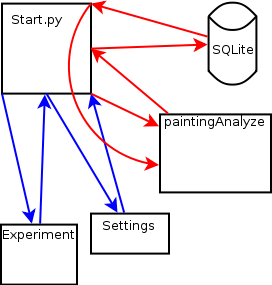
\includegraphics[scale=0.5]{afsnit/implementation/billeder/workflow_start_py.png}
	\end{center}
	\caption{De blå pile er ting, som sker en enkelt gang, mens de blå
	bliver gentaget indtil der ikke er flere billeder at arbejde på}
\end{figure}

\begin{lstlisting}[caption={Pseudokode for den naive metode},
    captionpos=b, label={pseudo_naiveMethod}, frame=tb,
    breaklines=false, float=h]
def NaiveMethod(image, settings):
    # Init ImageRegions dict
    ImageRegions = {}

    # Walk through all the CutRatios
    for CutRatio in settings:
        # Init RatioRegions dict
        RatioRegions = {}

        # Walk through every Cut in the ratio
        for Cut in CutRatio:
            # Set up the constraints, extract regions and prune the regions
            Constraints = new Constraints(image, Cut, settings)
            CutRegions = NaiveExtraction(image)
            InterestingRegions = GetInterestingRegions(CutRegions, Constraints)
            InterestingRegionsInCut =
                    GetInterestingRegionsInCut(InterestingRegionsInCut, Constraints)

            # Put the resulting instance of CutRegions
            # in the Regions-dict
            RatioRegions[Cut] = InterestingRegionsInCut

        # Put the resulting RatioRegions in the ImageRegions-dict
        ImageRegions[CutRatio] = RatioRegions

    # Return the resulting ImageRegions-dict
    return ImageRegions
\end{lstlisting}

\begin{lstlisting}[caption={Pseudokode til analyse af malerier efter
    metode}, captionpos=b, label={pseudo_naiveMethod}, frame=tb,
    breaklines=false, float=h]
def AnalysePainting(painting, settings):
    # Get the method used for the analysis
    method = settings.method

    # Use the right method
    if method == 'naive':
        image = painting.getImage()
        return NaiveMethod(image, settings)
    else:
        print 'No such method'
        return None
\end{lstlisting}

}
% vim: set tw=72 spell spelllang=da:

%Flow diagram (flot).
\subsection{Indstillinger}
Snak om indstillinger for de enkelte kørsler og globale indstillinger.

}

% vim: set tw=72 spell spelllang=da:
